
\setcounter{chapter}{4}
\chapter{Sprint 3: Checkout Integration}
\minitoc %insert la minitoc
\graphicspath{{Chapter5/figures/}}

%\DoPToC
%==============================================================================
\pagestyle{fancy}
\fancyhf{}
\fancyhead[R]{\bfseries\rightmark}
\fancyfoot[R]{\thepage}
\renewcommand{\headrulewidth}{0.5pt}
\renewcommand{\footrulewidth}{0pt}
\renewcommand{\chaptermark}[1]{\markboth{\MakeUppercase{\chaptername~\thechapter. #1 }}{}}
\renewcommand{\sectionmark}[1]{\markright{\thechapter.\thesection~ #1}}


\begin{spacing}{1.2}

\section*{Introduction}
In this chapter, we will implement the tools needed for developers to be able to integrate Flouci in their websites.

In order to make it portable in any existing e-commerce website, we decided to implement it in pure javascript.
\section{Front End Integration}
In this section, we will implement the front end payment plugin that  can be integrated in any HTML code.
\subsection{User Experience}
In the online payment, we faced a small issue regarding the payment experience, because the process is different from the mobile version. The online payments needs to wait until the developer accept the order.
So we decided to create the same QR code experience in mobile and only add a step to enter a six digits code in the browser.

Figure \ref{fig:onlinepay} shows the payment form of the developer API.
\begin{figure}[H]\centering
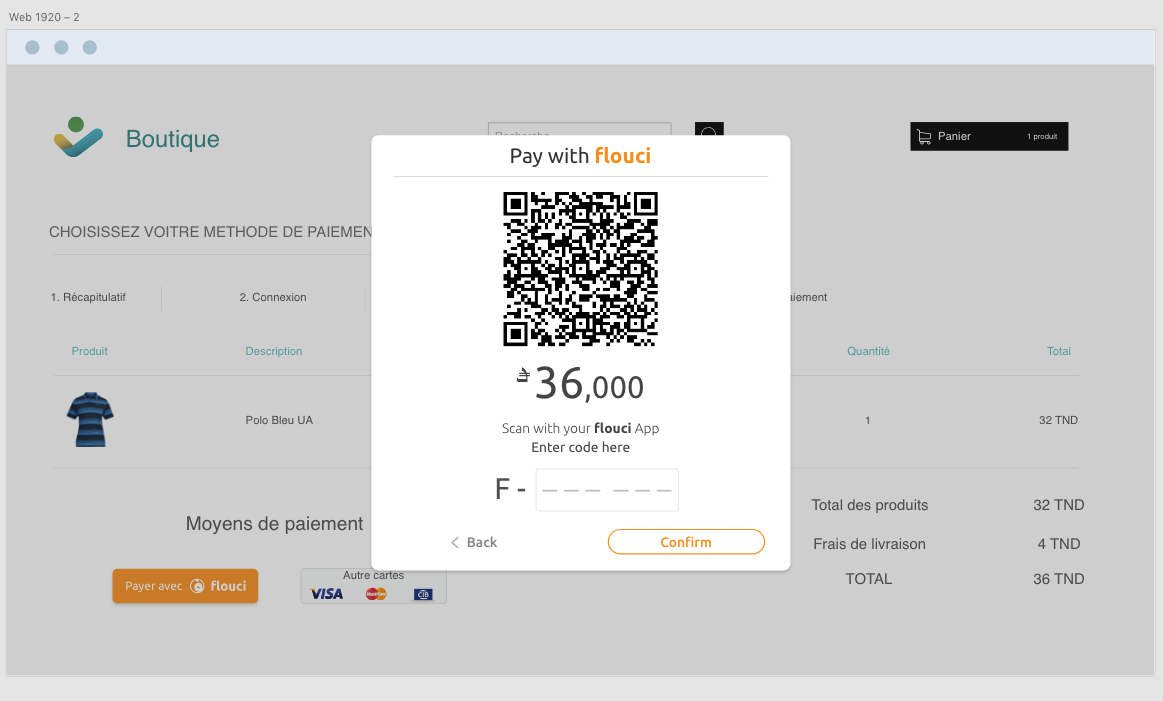
\includegraphics[width= \textwidth, keepaspectratio ]{Checkout_screen.png}
\caption{Flouci payment Form}
\label{fig:onlinepay}
\end{figure}

\subsection{Implementation}
To create our front-end form and make it easy to integrate, we created a web-pack project that bundles next generation javascript and CSS into one single javascript file.
The code contains the payment form and an API validation call to the payment API.
If the six-digit code entered by the user is correct, the script returns the code to the form submit action.
\subsection{Building The Script File}
Our front-end integration is basically a web script capable of delivering three main objectives:
\begin{itemize}
	\item \textbf{Payment Button:} The payment button should have a distinct and recognizable style across all e-commerce websites.
	\item \textbf{Payment Form:} The payment form goal is to encode the app public key, amount and other optional fields into one single QR code readable by our Flouci App.
	\item \textbf{Validation API:} After scanning the QR code, the script should be able to validate the pre-payment with the payments API and give feedback to the e-commerce backend.
\end{itemize}

In order to create this script, we had to use different modules such as a QR code generator. This made it impossible to write everything in vanilla javascript and deliver our project on time.


The solution we agreed on is to create a webpack project. With webpack, we could use next generation javascript and already existing NPM modules then bundle everything in one script.

The figure \ref{fig:webpack} shows how webpack can transform a javascript module with dependencies into one static bundle.
\begin{figure}[H]\centering
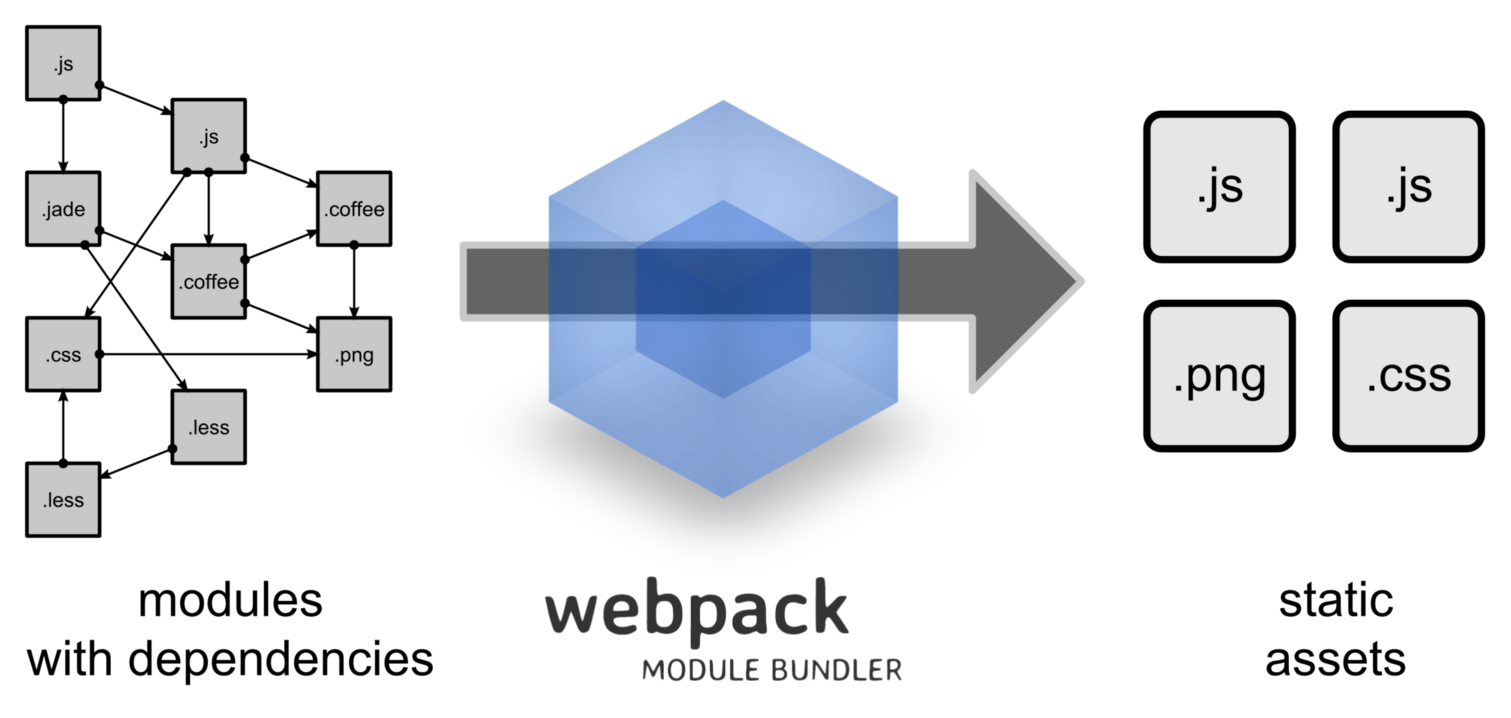
\includegraphics[width=\textwidth, keepaspectratio ]{webpack.png}
\caption{Webpack build process}
\label{fig:webpack}
\end{figure}

\subsection{Design Patterns}
In order to implement our solution, we faced a lot of design problems. Luckily such problems were commonly occurring problems in software design. So we studied the known design patterns \cite{designpattern} and we solved our issues with these design patterns:
\begin{itemize}
	\item \textbf{Creational design patterns \cite{designpattern}:} The QR code contains different fields so we followed the Builder design pattern to create it.
	\item \textbf{Structural design patterns \cite{designpattern}:} Our form hide different components and complex behavior so we implemented a Facade design pattern to deliver a single class that
	 represents the entire subsystem.
	 \item \textbf{Behavioral design patterns \cite{designpattern}:} The process of payments include different steps, that's why we implemented a  Chain of responsibility design pattern to pass the payment request between our three main objects.
\end{itemize}
\subsection{Integration}
After hosting the javascript file we can easily add the form to our project. The form will only require the public app key  and the amount.
The HTML code is listed in \ref{code:html}.
\begin{lstlisting}[rulecolor=\color{white}]
\end{lstlisting}
\begin{lstlisting}[label=code:html,caption=Flouci Integration Java,language=xml]
 <form id="myform" action="/handle_payment" method="post">
    <script
            src="https://developersdev.flouci.com/static/main.js"
            data-key="f6b5d0a5-e559-4acb-bcbb-a9e6ec9d788d"
            data-amount="2700000"
            data-name="Flouci Checkout"
            data-description="Flouci Data"

    </script>
  </form>
\end{lstlisting}


\section{Back End Integration}
After the user inputs the six digits code into the form, the form checks the validity of the payment and return a special key to the backend ( the action function inputed by the developer)

The developer then is only required to call an endpoint to accept the payment and then redirects the user to an other page depending on the payment result.

In the figure \ref{fig:flask} we show the code of a simple flask server with a Flouci integration that works with the HTML code listed in \ref{code:html}.
\begin{figure}[H]\centering
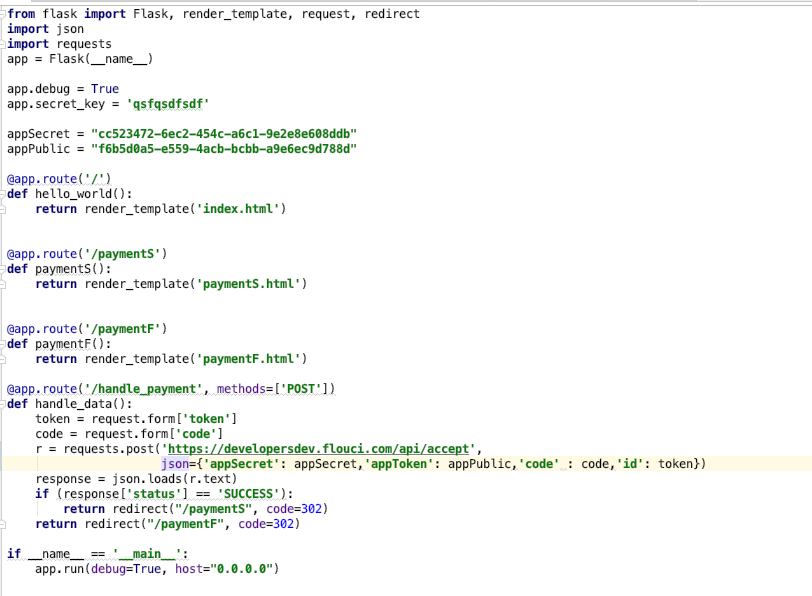
\includegraphics[width=\textwidth,height=12cm]{flask.png}
\caption{Flouci payment Backend Integration}
\label{fig:flask}
\end{figure}
\section{Payment Process}
To summarize the payment process, we created a sequence diagram prsented in the figure \ref{fig:FPSD} that contains all the interactions needed to process a payment.
\begin{figure}[H]\centering
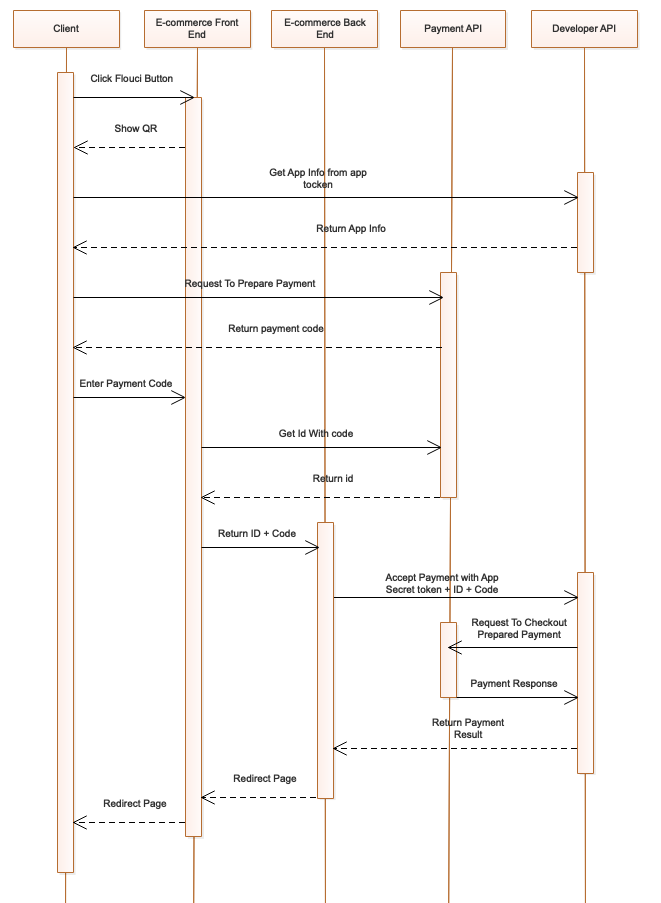
\includegraphics[width=\textwidth,height=18cm]{Payment_Sequence_Diagram.png}
\caption{Flouci Payment Sequence Diagram}
\label{fig:FPSD}
\end{figure}
In order to make a payment, the user should click the payment button and scan the QR code. The mobile app then gets the app info from the developer API and verify its validity. If the app is valid the mobile phone call the payment API to prepare the payment, this will return a key. The user inputs the key into the form and then the form will call the payment API to verify it and get an extra id to return it to the developer backend. Finally the developer should call the developer api and send his app secret, the key and the id returned by the form, the developer api calls the payment api to execute the payment and return the result to the developer.
\section*{Conclusion}
In this chapter we implemented the checkout API, which serve as an integration module that can be integrated in any web based project.

In the implementation of our solution we had to made it the simplest integration possible and the most portable one. And we made as easy as implementing a simple REST call.

With the checkout integration module, we finally have all the pieces needed in the Flouci online payment process. We now have a fully functional project.

\end{spacing}
